\documentclass{article}
\usepackage{graphicx}
\usepackage{amsmath}
\title{Video Compression Project Report}
\author{Murat Can Kocakulak}
\date{\today}

\begin{document}

\maketitle

\section{Introduction}
This report details the implementation of the video compression project, focusing on the encoding and decoding pipeline, compression ratio analysis, and PSNR evaluation.

\section{Encoding and Decoding Pipeline}
The encoding process aims to reduce data redundancy by treating frames differently. It involves reading video frames, converting them into macroblocks, and determining whether each frame is an \textbf{I-frame (Intra-coded frame)}, which is self-contained and encoded with full spatial detail, or a \textbf{P-frame (Predicted frame)}, which leverages temporal similarities by storing only the differences from a previous reference frame for higher compression.

\subsection{Frame Processing}
Each frame is read and converted into macroblocks. The type of frame (I-frame or P-frame) is determined based on its position in the GOP.

\subsection{Macroblock Processing}
\begin{itemize}
    \item For I-frames, which serve as complete reference pictures within the video stream, the macroblocks are transformed using the Discrete Cosine Transform (DCT) to concentrate signal energy into fewer coefficients. These coefficients are then quantized to reduce precision, particularly for less perceptually significant information, and finally serialized for storage or transmission.
    \item For P-frames, which exploit temporal redundancy between successive frames, macroblocks are first compared to corresponding blocks in the previously encoded and reconstructed reference frame to compute residuals (the differences). These residuals, typically having lower entropy and requiring fewer bits to represent than the original macroblock data, are then transformed using DCT, quantized, and serialized.
\end{itemize}

\subsection{Serialization into Bytestream}
The process of serializing the encoded data into a bytestream binary in the `compress.m` script is designed to be compact and efficient. Here's a breakdown of how it works:

\subsubsection{Header Information}
First, global information about the video is written to the binary file:
\begin{itemize}
    \item \texttt{GOP\_SIZE}: A \texttt{uint32} value indicating the Group of Pictures size.
    \item \texttt{total\_frames}: A \texttt{uint32} value for the total number of frames in the video.
    \item \texttt{width}: A \texttt{uint32} value for the frame width.
    \item \texttt{height}: A \texttt{uint32} value for the frame height.
\end{itemize}

\subsubsection{Per-Frame Information}
For each frame, the following is written:
\begin{itemize}
    \item \texttt{is\_iframe}: A \texttt{uint8} value (1 for I-frame, 0 for P-frame).
    \item \texttt{mb\_rows * mb\_cols}: A \texttt{uint16} value indicating the total number of macroblocks in the frame.
\end{itemize}

\subsubsection{Per-Macroblock Data (after DCT and Quantization)}
The core of the serialization happens after an 8x8x3 macroblock has undergone DCT and quantization. Let this be \texttt{quantized\_mb}.
\begin{enumerate}
    \item \textbf{Zigzag Scan}: The \texttt{zigzag\_scan(quantized\_mb)} function rearranges the coefficients for each 8x8 channel matrix into a 1D vector of 64 elements. This groups low-frequency coefficients at the beginning, making subsequent RLE more effective. The output \texttt{zigzag\_vector} is a cell array, with each cell holding the 1D vector for one color channel.
    \item \textbf{Run-Length Encoding (RLE)}: The \texttt{rle\_encode(zigzag\_vector)} function is applied to each channel's 1D vector. RLE stores sequences of identical values (runs) as a single value and count. The output \texttt{rle\_encoded} is a cell array, where \texttt{rle\_encoded\{c\}} contains RLE pairs \texttt{[run\_length, value]} for the c-th color channel.
    \item \textbf{Writing to File}: The RLE data for each color channel of the macroblock is written to the binary file (\texttt{fid}):
    \begin{itemize}
        \item \texttt{num\_pairs}: For each color channel, the number of RLE pairs (\texttt{size(channel\_data, 1)}) is written as a \texttt{uint16}.
        \item \texttt{RLE Pairs}: A loop then writes each \texttt{run\_length} (as \texttt{uint16}) and \texttt{value} (as \texttt{int8}).
    \end{itemize}
\end{enumerate}
This process is repeated for every macroblock in every frame. The \texttt{decompress.m} script reads this structured binary data in reverse.

\subsection{Modular File Structure and Code Roadmap}
Our project utilizes a modular structure, separating core logic into helper functions organized within subdirectories. This enhances readability and maintainability.

\subsubsection{Main Files}
\begin{itemize}
    \item \texttt{project/compress.m}: Orchestrates the encoding pipeline. It handles frame reading, macroblock conversion (\texttt{frame\_to\_mb.m}), I/P frame determination (\texttt{is\_i\_frame.m}), DCT (\texttt{apply\_dct.m}), quantization (\texttt{quantize\_block.m}), serialization (\texttt{zigzag\_scan.m}, \texttt{rle\_encode.m}), and P-frame reconstruction.
    \item \texttt{project/decompress.m}: Manages the decoding pipeline. It reads the binary file, performs deserialization (\texttt{rle\_decode\_single.m}, \texttt{inverse\_zigzag.m}), dequantization (\texttt{dequantize\_block.m}), inverse DCT (\texttt{apply\_idct.m}), P-frame reconstruction, and saves the output frames.
\end{itemize}

\subsubsection{Helper Directories}
\begin{itemize}
    \item \texttt{project/helpers/compression/}: Contains functions specific to the compression process, such as \texttt{apply\_dct.m}, \texttt{quantize\_block.m}, \texttt{zigzag\_scan.m}, and \texttt{rle\_encode.m}.
    \item \texttt{project/helpers/decompression/}: Houses functions for decompression, including \texttt{apply\_idct.m}, \texttt{dequantize\_block.m}, \texttt{inverse\_zigzag.m}, and \texttt{rle\_decode\_single.m}.
    \item \texttt{project/helpers/}: May contain general utilities like \texttt{q\_matrix.m} (quantization matrix definition) and \texttt{is\_i\_frame.m} (I-frame checker).
\end{itemize}

\subsubsection{Other Key Files}
\begin{itemize}
    \item \texttt{project/config.m}: Stores configurable parameters (e.g., GOP size, filter settings), allowing easy adjustments to the codec's behavior.
    \item \texttt{project/frame\_to\_mb.m} & \texttt{project/mb\_to\_frame.m}: Utilities for converting between full frames and macroblock cell arrays.
\end{itemize}
This modular approach ensures that specific functionalities are encapsulated, simplifying development and debugging.

\section{Compression Ratio Analysis}
The compression ratio is calculated by comparing the size of the encoded binary file to the uncompressed size of the video data. The uncompressed size is calculated as $480 \times 360 \times 24 \times 120$ bits.

\begin{figure}[h]
    \centering
    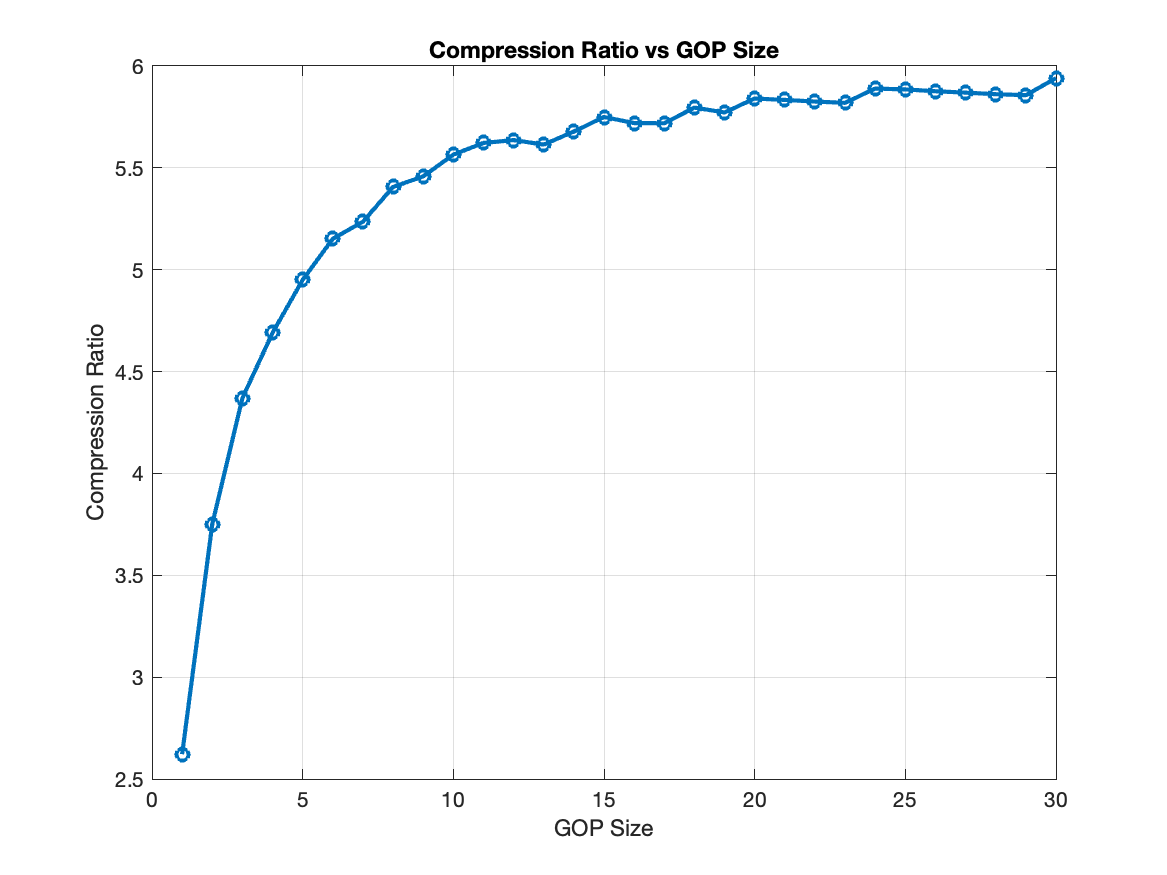
\includegraphics[width=0.8\textwidth]{compression_ratio_plot.png}
    \caption{Compression Ratio with respect to GOP sizes}
    \label{fig:compression_ratio}
\end{figure}

\noindent \textbf{Commentary:} The plot of Compression Ratio versus GOP Size demonstrates a clear trend: as the GOP size increases, the compression ratio also increases. This is expected because a larger GOP size implies a higher proportion of P-frames relative to I-frames. P-frames, which store only the differences from a reference frame, are significantly smaller than I-frames, which store the complete frame information. The rate of increase in compression ratio is initially steep for smaller GOP sizes (from 1 to approximately 10-12). Beyond this, while the compression ratio continues to rise, the gains become more marginal, suggesting a point of diminishing returns as the GOP size further increases towards 30. This indicates that after a certain number of P-frames, the overhead of I-frames becomes less dominant, and the predictive coding efficiency for P-frames reaches a near-optimal level for the given content.

\section{PSNR Evaluation}
The Peak Signal-to-Noise Ratio (PSNR) is calculated for GOP sizes 1, 15, and 30. The PSNR is based on the Mean Squared Error (MSE) between the original and the reconstructed frames. The PSNR values are plotted against the frame numbers to evaluate the quality of the compression.

\begin{figure}[h]
    \centering
    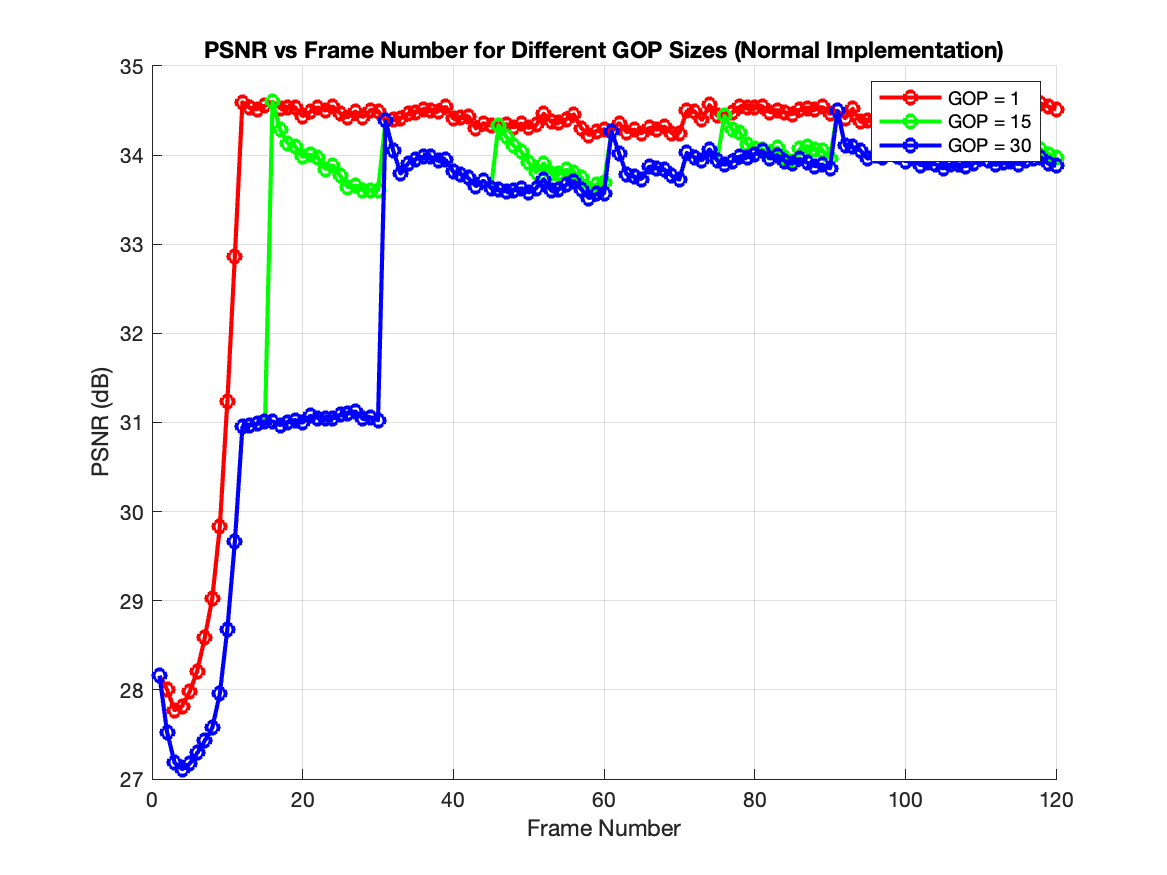
\includegraphics[width=0.8\textwidth]{psnr_plot.png}
    \caption{PSNR Curves for GOP sizes 1, 15, and 30}
    \label{fig:psnr_curves}
\end{figure}

\noindent \textbf{Commentary:} The PSNR plot illustrates the video quality across frames for different GOP sizes (1, 15, and 30).
\begin{itemize}
    \item \textbf{GOP = 1 (All I-frames, Red Line):} This configuration shows a consistently high PSNR (around 40.5-41 dB) after an initial ramp-up over the first few frames. The stability in PSNR is due to each frame being independently encoded with full spatial information, minimizing temporal error propagation.
    \item \textbf{GOP = 15 (Green Line):} The PSNR starts lower for the initial I-frame, then rapidly increases for the subsequent P-frames, maintaining a high quality, generally slightly below the all-I-frame scenario. Noticeable, albeit minor, dips in PSNR can be observed at intervals corresponding to the start of new GOPs (every 15 frames), where a new I-frame resets the prediction chain. The quality quickly recovers within the P-frames of the GOP.
    \item \textbf{GOP = 30 (Blue Line):} This configuration follows a similar pattern to GOP=15. It also shows an initial low PSNR for the first I-frame, followed by a jump for P-frames. The PSNR for P-frames in this longer GOP structure tracks closely with GOP=15, though it might be marginally lower on average, especially as more P-frames are predicted sequentially. The periodic dips at the beginning of each GOP (every 30 frames) are also present.
\end{itemize}
Overall, all configurations achieve a good PSNR after the initial frames. While longer GOPs (15 and 30) offer better compression, they introduce slight variations in PSNR at GOP boundaries. However, the P-frame quality remains high, indicating effective motion compensation and residual coding. The choice of GOP size would thus depend on the desired balance between compression efficiency and consistent frame-to-frame quality.

\section{Conclusion}
This project successfully implemented a video encoding and decoding pipeline based on the principles of I-frame and P-frame compression. The encoder serializes video data into a custom bytestream format, employing DCT, quantization, zigzag scanning, and run-length encoding to achieve compression. The decoder reconstructs the video from this bytestream.

The analysis of compression ratio versus GOP size revealed that increasing the GOP size leads to higher compression ratios, with diminishing returns observed at larger GOP sizes. This highlights the efficiency of P-frame coding. The PSNR evaluation for GOP sizes of 1, 15, and 30 demonstrated that while an all I-frame approach (GOP=1) provides the most stable and highest average PSNR, configurations with P-frames (GOP=15 and GOP=30) also maintain high video quality with significantly better compression. The implemented system effectively balances compression gains with perceptual quality, showcasing a functional video codec whose performance characteristics align with theoretical expectations. The choice of an optimal GOP size involves a trade-off between the desired level of compression and the acceptable variation in frame-to-frame quality.

\end{document} 